\newcommand{\sketchtextsize}{\fontsize{8pt}{8pt}\selectfont}

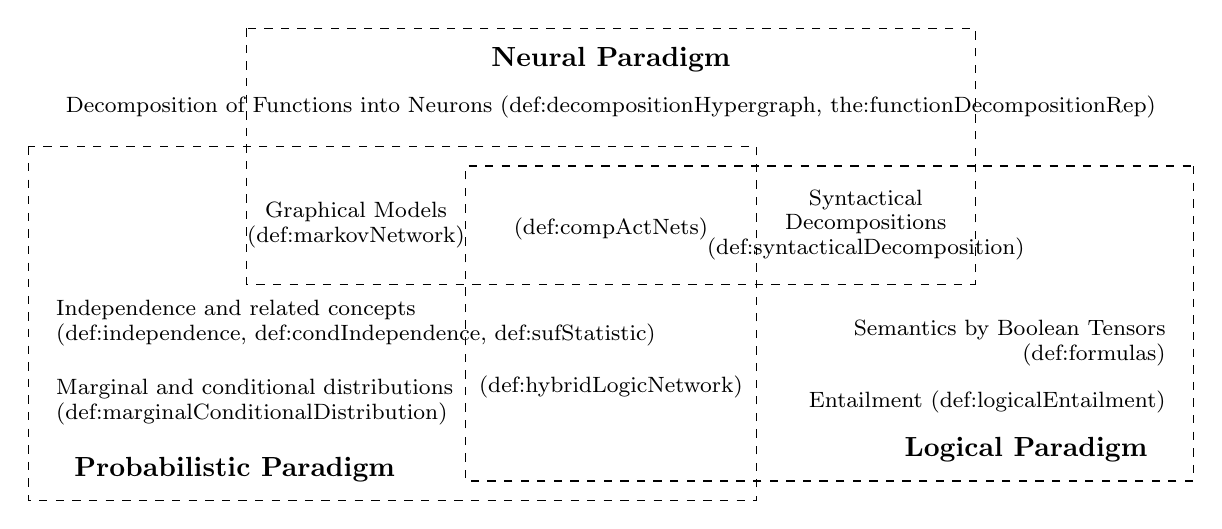
\begin{tikzpicture}[yscale=1, xscale=0.925]

    \node[anchor=center] at (0,0.1) {\bf Neural Paradigm};
    \draw[dashed] (-5,0.5) rectangle (5,-2.75);
    \node[anchor=center] at (0,-0.5) {
        \sketchtextsize Decomposition of Functions into Neurons (\defref{def:decompositionHypergraph}, \theref{the:functionDecompositionRep})};

    \node[anchor=west] at (-7.5,-5.1) {\bf Probabilistic Paradigm};
    \draw[dashed] (-8,-1) rectangle (2,-5.5);
    \node[anchor=west, align=left] at (-7.75,-3.25) {
        \sketchtextsize Independence and related concepts \\[-3pt]
        \sketchtextsize (\defref{def:independence}, \defref{def:condIndependence}, \defref{def:sufStatistic})};
    \node[anchor=west, align=left] at (-7.75,-4.25) {
        \sketchtextsize Marginal and conditional distributions \\[-3pt]
        \sketchtextsize (\defref{def:marginalConditionalDistribution})};


    \node[anchor=east] at (7.5,-4.85) {\bf Logical Paradigm};
    \draw[dashed] (8,-1.25) rectangle (-2,-5.25);
    \node[anchor=east, align=right] at (7.75,-3.5) {
        \sketchtextsize Semantics by Boolean Tensors \\[-3pt]
        \sketchtextsize (\defref{def:formulas})};
    \node[anchor=east, align=right] at (7.75,-4.25) {
        \sketchtextsize Entailment (\defref{def:logicalEntailment})};

    \node[anchor=center, align=center] at (-3.5,-2) {
        \sketchtextsize Graphical Models \\[-3pt]
        \sketchtextsize (\defref{def:markovNetwork})};

    \node[anchor=center, align=center] at (3.5,-2) {
        \sketchtextsize Syntactical \\[-3pt]
        \sketchtextsize Decompositions \\[-3pt]
        \sketchtextsize (\defref{def:syntacticalDecomposition})};

    \node[anchor=center, align=center] at (0,-2) {
        \sketchtextsize \CompActNets{} \\[-3pt]
        \sketchtextsize (\defref{def:compActNets})};

    \node[anchor=center, align=center] at (0,-4) {
        \sketchtextsize \HybridLogicNetworks{} \\[-3pt]
        \sketchtextsize (\defref{def:hybridLogicNetwork})};


%	\node[anchor=center] (text) at (-2.25,13) {Distributions with sufficient statistic $\formulaset$: $\realizabledistsof{\formulaset,\maxgraph}$};
%	\draw[dashed] (-10.5,14) rectangle (5,6);
%
%	\draw[dashed] (-10,12) rectangle (4.5,6.5);
%	\node[anchor=center] (text) at (-2.25,11) {\HybridLogicNetworks{}: $\realizabledistsof{\formulaset,\elgraph}$};
%
%	\draw[\probcolor] (-9.5,10) rectangle (-3,7);
%	\node[\probcolor] (text) at (-6,9) {\MarkovLogicNetworks{}: };
%	\node[\probcolor] (text) at (-6,7.9) {Positive activation cores};
%
%	\draw[\concolor] (-2.5,10) rectangle (4,7);
%	\node[\concolor] (text) at (1,9) {\HardLogicNetworks{}:};
%	\node[\concolor] (text) at (1,7.9) {Boolean activation cores};

\end{tikzpicture}